\documentclass[]{article}

\usepackage[utf8]{inputenc}
\usepackage[paperheight=1.5in,paperwidth=4.4in,margin=0in]{geometry}
\usepackage{tikz}
\usetikzlibrary{shapes,arrows,automata,calc}
\usepackage{color}

\usepackage{booktabs}  % nicer table borders 

\begin{document}

%\clearpage
%\thispagestyle{empty}

\tiny{
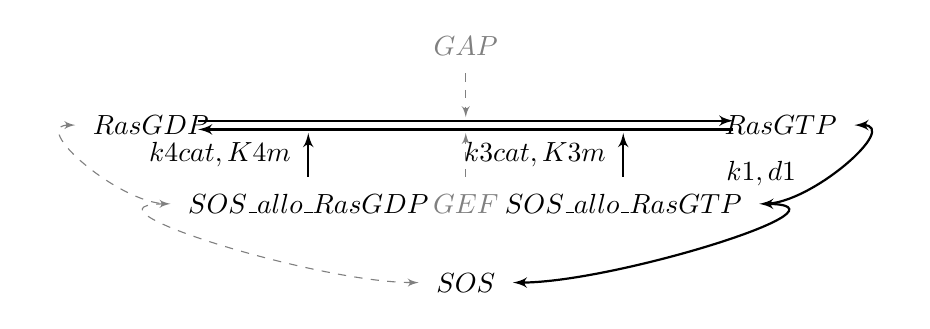
\begin{tikzpicture}[auto, outer sep=3pt, node distance=0cm,>=latex']

\node [gray] at (-6.1, 7) (GAP) {$GAP$};

\node  at (-10.1, 6) (RASGDP) {$RasGDP$};
%\node  at ($(R)!0.5!(RS)$) (RRS) {};
%\draw [<->, thick] ($(R)+(+.1,0)$) to node {$k_2, k_3$} ($(RS)+(-0.2, 0)$);
%\draw [<-, thick] (S) edge[in=180, out=330] (RRS);
%\node  at (-3.8, 7.8) (X3) {$k_4^{cat},K_4m$};

\node at (-2.1, 6) (RASGTP) {$RasGTP$};
%\draw [->, thick] ($(RS)+(+.2,0)$) to node {$k_4$} ($(Rpp)+(-0.3, 0)$);


\node [gray] at (-6.1, 5) (GEF) {$GEF$};
\node at (-4.1, 5) (SOSGTP) {$SOS\_allo\_RasGTP$};
\node at (-8.1, 5) (SOSGDP) {$SOS\_allo\_RasGDP$};

\node at (-6.1, 4) (SOS) {$SOS$};

%\draw [<-, thick] (RASGTP) edge (RASGDP);
\draw [->, thick] ($(RASGTP)-(0.6, 0.055)$) -- ($(RASGDP)-(-0.6, 0.055)$);
\draw [<-, thick] ($(RASGTP)-(0.6, -0.055)$) -- ($(RASGDP)-(-0.6, -0.055)$);

\node  at (-2.1, 5) (MIDR) {};
\draw [->, thick] (MIDR) to node[above] {$k1, d1$} (SOSGTP);
\draw [<-, thick] (RASGTP) edge[out=0, in=0] ($(MIDR)-(.2, 0)$);
\draw [<-, thick] (SOS) edge[out=0, in=0] ($(MIDR)-(.2, 0)$);

\node  at (-10.1, 5) (MIDL) {};
\draw [->, dashed, gray] (MIDL) to node[above] {} (SOSGDP);
\draw [<-, dashed, gray] (RASGDP) edge[out=180, in=180] ($(MIDL)+(.2, 0)$);
\draw [<-, dashed, gray] (SOS) edge[out=180, in=180] ($(MIDL)+(.2, 0)$);

\draw [->, thick] (SOSGDP) to node {$k4cat, K4m$} ($(-8.1, 5.9)$);
\draw [->, thick] (SOSGTP) to node {$k3cat, K3m$} ($(-4.1, 5.9)$);

\draw [->, dashed, gray] (GAP) to node {} ($(-6.1, 6.1)$);
\draw [->, dashed, gray] (GEF) to node {} ($(-6.1, 5.9)$);



\end{tikzpicture} 
}

\end{document}

